% 修士学位論文
%
% 研究題目: 雷雲を想定した強制により生じるガス惑星表層流の数値計算
%
% 作成者: 鈴木 綾馬
% 作成日: 2021/01/02
%
%%%%%%%%%%%%%%%%%%%%%%%%%%%%%%%%%%%%%%%%%%%%%%%%%%%%%%%%
%%%%%%%%             Style  Setting             %%%%%%%%
% フォント: 12point (最大), 片面印刷
\documentclass[a4j,12pt,openbib,oneside]{jreport}

%%%%%%%%%%%%%%%%%%%%%%%%%%%%%%%%%%%%%%%%%%%%%%%%%%%%%%%%
%%%%%%%%             Package Include            %%%%%%%%
\usepackage{ascmac}
\usepackage{tabularx}
\usepackage[dvipdfmx]{graphicx}
\usepackage{amssymb}
\usepackage{amsmath}
\usepackage{mathrsfs}
\usepackage{Dennou6}            % 電脳スタイル ver 6
\usepackage{bm}
\usepackage{framed}
\usepackage[dvipdfmx]{color}
\usepackage{empheq}
\usepackage{comment}
\usepackage{fancybox}
\usepackage{enumitem}
\usepackage{mathtools}
\usepackage{listliketab}
\usepackage[stable]{footmisc}
\usepackage{setspace}
\usepackage[dvipdfmx]{hyperref}
\usepackage{pxjahyper} % 日本語対応 (使わないともくじ部分が文字化けする)
\usepackage{url}
\usepackage[numbers,sort]{natbib}
%\usepackage[biblabel]{cite} % natbib と衝突する可能性があるので使わないことにする
\usepackage{remreset}
\usepackage{subfigure}
\usepackage{here} % 強制的に画像位置を指定

%%%%%%%%%%%%%%%%%%%%%%%%%%%%%%%%%%%%%%%%%%%%%%%%%%%%%%%%
%%%%%%%%            PageStyle Setting           %%%%%%%%
\pagestyle{DAmyheadings}
%%%%%%%%%%%%%%%%%%%%%%%%%%%%%%%%%%%%%%%%%%%%%%%%%%%%%%%%
%%%%%%%%        Title and Auther Setting        %%%%%%%%
%%
%%  [ ] はヘッダに書き出される.
%%  { } は表題 (\maketitle) に書き出される.
\Dtitle{修士学位論文}
\Dauthor{鈴木 綾馬}
\Ddate{2020/01/29}       % 提出期限日
\Dfile{rsuzuki\_Mthesis.tex}

%%%%%%%%%%%%%%%%%%%%%%%%%%%%%%%%%%%%%%%%%%%%%%%%%%%%%%%%
%%%%%%%%   Set Counter (chapter, section etc. ) %%%%%%%%
\setcounter{chapter}{0}    % 章番号
\setcounter{section}{2}    % 節番号
\setcounter{subsection}{0} % 小節番号
\setcounter{equation}{0}   % 式番号
\setcounter{page}{0}       % 開始ページ番号
\setcounter{figure}{0}     % 図番号
\setcounter{table}{0}      % 表番号
%\setcounter{footnote}{0}

%%%%%%%%%%%%%%%%%%%%%%%%%%%%%%%%%%%%%%%%%%%%%%%%%%%%%%%%
%%%%%%%%        Counter Output Format           %%%%%%%%
\def\thechapter{\arabic{chapter}}
\def\thesection{\arabic{chapter}.\arabic{section}}
\def\thesubsection{\arabic{chapter}.\arabic{section}.\arabic{subsection}}
\def\theequation{\arabic{equation}}
\def\thepage{\arabic{page}}
\def\thefigure{\arabic{figure}}
\def\thetable{\arabic{table}}
\def\thefootnote{*\arabic{footnote}}
%%%%%%%%%%%%%%%%%%%%%%%%%%%%%%%%%%%%%%%%%%%%%%%%%%%%%%%%
%%%%%%%%        Dennou-Style Definition         %%%%%%%%

%% 改段落時の空行設定
\Dparskip      % 改段落時に一行空行を入れる
%\Dnoparskip    % 改段落時に一行空行を入れない

%% 改段落時のインデント設定
\Dparindent    % 改段落時にインデントする
%\Dnoparindent  % 改段落時にインデントしない

%%%%%%%%%%%%%%%%%%%%%%%%%%%%%%%%%%%%%%%%%%%%%%%%%%%%%%%%%%
%% Macro defined by author
\def\univec#1{ \hat{ \Dvect{\rm #1}} }
\def\DD#1#2{\frac{\mathrm D #1}{\mathrm D #2}}
\def\dd#1#2{\frac{\mathrm d #1}{\mathrm d #2}}
\def\Dd#1{\; {\mathrm d} #1}
\def\D#1{\Dvect{#1}}
\def\p{\prime}
\renewcommand{\DP}[3][]{\frac{\partial^{#1} #2}{\partial #3^{#1}}}
\def\ol#1{\overline{#1}}
\def\wh#1{\widehat{#1}}
\def\wt#1{\widetilde{#1}}

\hypersetup{
  colorlinks,
  citecolor=red,
  linkcolor=blue,
  urlcolor=blue
}
\bibpunct{(}{)}{,}{a}{,}{,}

\makeatletter
\@removefromreset{figure}{chapter}
\def\thefigure{\arabic{figure}}

\@removefromreset{table}{chapter}
\def\thetable{\arabic{table}}

\@removefromreset{equation}{chapter}
\def\theequation{\arabic{equation}}

\@removefromreset{footnote}{chapter}
\def\thefootnote{\arabic{footnote}}

%\@removefromreset{subfigure}{chapter}
%\def\thesubfigure{(\alph{subfigure})}
%\def\p@subfigure{\arabic{figure}}
%\@removefromreset{subtable}{chapter}
%\def\thesubtable{(\alph{subtable})}
%\def\p@subtable{\arabic{table}}
%最新の TeX では \subfigure, \subtable は廃止されている。(代替コマンド: \subcaption)
%\makeatother

\renewcommand\thefootnote{*\arabic{footnote}}
%%%%%%%%%%%%%%%%%%%%%%%%%%%%%%%%%%%%%%%%%%%%%%%%%%%%%%%%
%%%%%%%%             Text Start                 %%%%%%%%


\begin{document}
\begin{titlepage}
 \centering
 \vspace*{40truept}
 {\Huge 修 \hspace{10pt} 士 \hspace{10pt} 学 \hspace{10pt} 位
 \hspace{10pt} 論 \hspace{10pt} 文}\\  % タイトル
 \vspace*{50truept}
 \textbf{{\Huge 雷雲を想定した強制により生じる\\
巨大惑星表層流の数値計算}} \\ % タイトル
 \vspace{30truept}
 \vspace{150truept}
 \begin{center}
  {\Large 北海道大学 理学院 宇宙理学専攻}
  \vspace{10truept}\\
  {\Large 惑星宇宙グループ 地球流体力学研究室}
  \vspace{10truept}\\
  {\Large 学籍番号 : 15S2015} 
  \vspace{30truept}\\
  {\LARGE 鈴木 綾馬}
  \vspace{10truept}
 \end{center}
 \begin{center}
  {\Large 2021 年 1 月 29 日}
 \end{center}
 \vspace{50truept}
 {\Large 北海道大学大学院理学院修士課程} \\
\end{titlepage}

%\maketitle

\thispagestyle{empty}
\setcounter{page}{0}

\clearpage
\begin{center}
\large{\bf 要旨}
\end{center}
\thispagestyle{empty}
\setcounter{page}{0}
ddd

\clearpage
\thispagestyle{empty}
\setcounter{page}{0}
\tableofcontents 
\thispagestyle{empty}
\setcounter{page}{0}

\clearpage
\setcounter{table}{0}
\setcounter{figure}{0}

\chapter{はじめに}
\section{巨大惑星表層流の特徴}
\label{sec:intro1}
巨大惑星
%
\footnote{ここで,巨大惑星とは
組成の主体が水素やヘリウムといった
ガスである巨大ガス惑星(木星,土星)と
それに比べ,水やメタンを多く含む
巨大氷惑星(天王星,海王星)の総称として用いる.}
%
大気の大規模循環とバンド構造は1970年代にPioneer,Voyger といった
探査機によって,これらの惑星の高解像度画像が撮影されて以来,
大きな謎となっている.
%
巨大惑星表層のの風速分布を図\ref{fig1}に示す\citep{showman2009atmospheric}.
%
風速分布の大きな特徴として,
巨大ガス惑星(木星,土星)では赤道域で
幅の広い西風とバンド構造に対応した中緯度域の縞状構造,
一方,巨大氷惑星では赤道域の幅の広い
東風が見られ,縞状構造は見られないといった特徴がある.
%
%
\begin{figure}[h]
  \begin{center}
    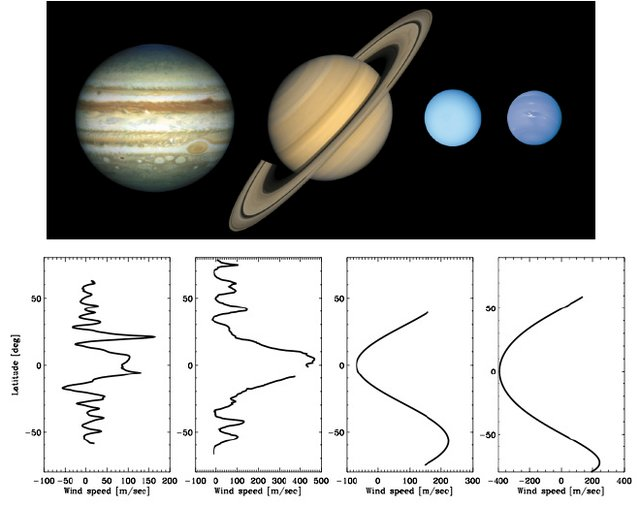
\includegraphics[clip,width=9cm]{./fig/intro/fig1.jpg}
    \caption{
      \footnotesize{上段 : 木星,土星,
天王星,海王星の可視光領域画像.
下段 : 縦軸が緯度,横軸が
クラウドトラッキングによって得られた
東西平均した東西風速分布.
巨大ガス惑星(木星,土星)は赤道域で幅の広い西風と
中緯度で東風/西風ジェットが交互に
約20個の縞状構造を形成しているのに対し,
巨大氷惑星(天王星,海王星)は
赤道域で幅の広い東風ジェットを含め
3つのジェットを形成している
\citep{showman2009atmospheric}.
      }
    }
    \label{fig1}
  \end{center}
\end{figure}
\clearpage
%
一方,極域の観測では
低中緯度ではあまり見られない空間スケールの大きい
低気圧性渦(自転と同じ向きに回転する渦)が
存在し,そのレジームが巨大惑星ごとに
異なることが近年のJuno, Cassini といった探査機の観測によってわかっている.
%
図\ref{fig2} に木星と土星の極域観測を示した.
木星では複数の低気圧性渦が極付近にある低気圧性渦を
取り囲んでいることがわかっている.
%
北極域では極から約$0.5^\circ$ 離れた位置に
低気圧性渦があり,その渦の周りを
8つの低気圧性渦が囲んでいる.
それぞれの渦の半径は約2000 - 2300 km(緯度幅で$\sim 2^\circ$) である.
%
南極域では極から約$1 \sim 2 ^\circ$ 離れた位置に
低気圧性渦があり,その渦の周りを
5つの低気圧性渦が囲んでいる.
それぞれの渦の半径は北極域のものより大きく,
約2800 - 3500 km(緯度幅で$\sim 3^\circ$) である\citep{Adriani2018}.
%
複数の低気圧性渦が存在する木星に対し,
土星では半径約2000 km(緯度幅で$\sim 2^\circ$) の
単一の低気圧性渦が各極域を支配している.
%
天王星,海王星もVoyger 2号と地上観測から
土星の低気圧性渦よりもサイズの大きい,
単一の低気圧性極渦(緯度幅で$\sim 10^\circ$)が存在していることが
示唆されている.
%
\begin{figure}[t]
  \begin{center}
    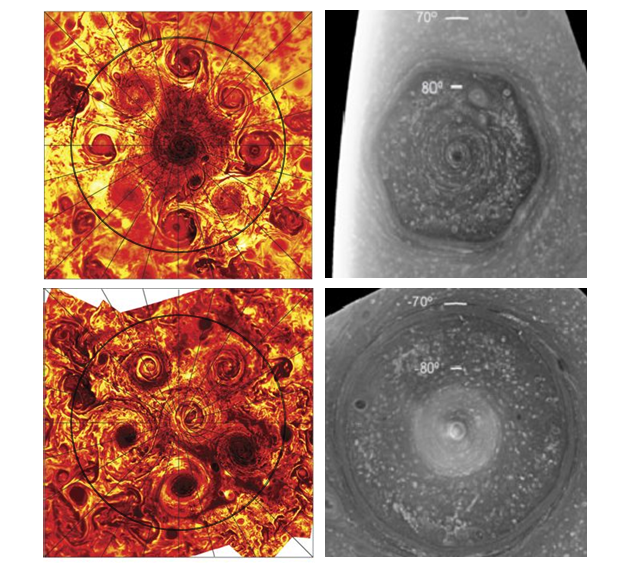
\includegraphics[clip,width=10cm]{./fig/intro/fig2.png}
    \caption{
      \footnotesize{左はJuno による木星観測(波長 : $5 \rm{\mu m}$).
黒の等緯度線は$80^\circ$ \citep{Adriani2018}.
右はCassini による土星観測(波長 : 750 nm) \citep{Antuano2015}.
上は北極域,下は南極域である.
      }
    }
    \label{fig2}
  \end{center}
\end{figure}
%
%
\section{先行研究}
\label{sec:intro2}
巨大惑星の内部構造の観測が難しいこともあり,
数値計算を行い,\ref{sec:intro1}節で
述べた表層流の特徴の再現を通して,理解を試みてきた.
%
しかし,巨大惑星の内部構造は内部熱源があることなど,
地球型惑星の内部構造と大きく異なっており,
地球大気とのアナロジーで観測される表層流を理解することは難しい.
特に,数値計算を行う際に問題になるのは
表層流の主となるエネルギー源は何なのかということである.
これについては大きく分けて,2つの説が考えられている.
%
1つは惑星内部の対流層と観測可能な雲が存在する大気上層部の
大気の運動が直接つながっているとする「深いモデル」である.
このモデルにおいては比較的,赤道域で強い西風ジェットは
形成されるものの,中高緯度域の縞状構造が発達しないという
問題点がある\citep{CHRISTENSEN2002}.
%
もう1つは,惑星深部の対流と大気上層部の対流は独立しており,
深部からの強制はあるものの深部の対流とは別のメカニズムで
構造が形作られているという「浅いモデル」である.
このモデルでは比較的,中高緯度の縞状構造が形成されるが,
赤道での西風ジェットが形成しないという問題点がある\citep{Scott2007}.
%
現在のところ決定的な議論は出来ていない.
%
\subsection{Showman et al. (2007)}
\label{sec:intro21}
これまでの「浅いモデル」の研究では
初期に小スケールの乱流を与え,時間発展をみる
自由減衰乱流実験\citep{Yoden1993}や
小規模な渦度強制を加える実験\citep{Scott2007}が行われてきた.
%
しかし,このような全球的かつ連続的な
強制が巨大惑星に働いているとは考えにくい.
%
擾乱を引き起こす現象として
木星,土星で観測されている雷雲(\cite{Gierasch2000}, \cite{Porco2005})が考えられている.
\cite{Showman2007}はこの雷雲を想定した
局所的かつ離散的な強制を与え,球面浅水実験を行った.
彼らは緯度$0 - 70^\circ$,経度$0 - 120^\circ$の範囲の領域を計算した.
その結果,中緯度の変形半径が小さい場合($< 2000$ km) には図\ref{fig3} のように
赤道域で幅の広い東風ジェットが形成し,
中緯度では渦が支配的になることがわかった.
%
中緯度の変形半径が4000 km より大きい場合には,
弱い渦は伴うものの,ジェットが支配的になることがわかった.
%
\begin{figure}[H]
  \begin{center}
    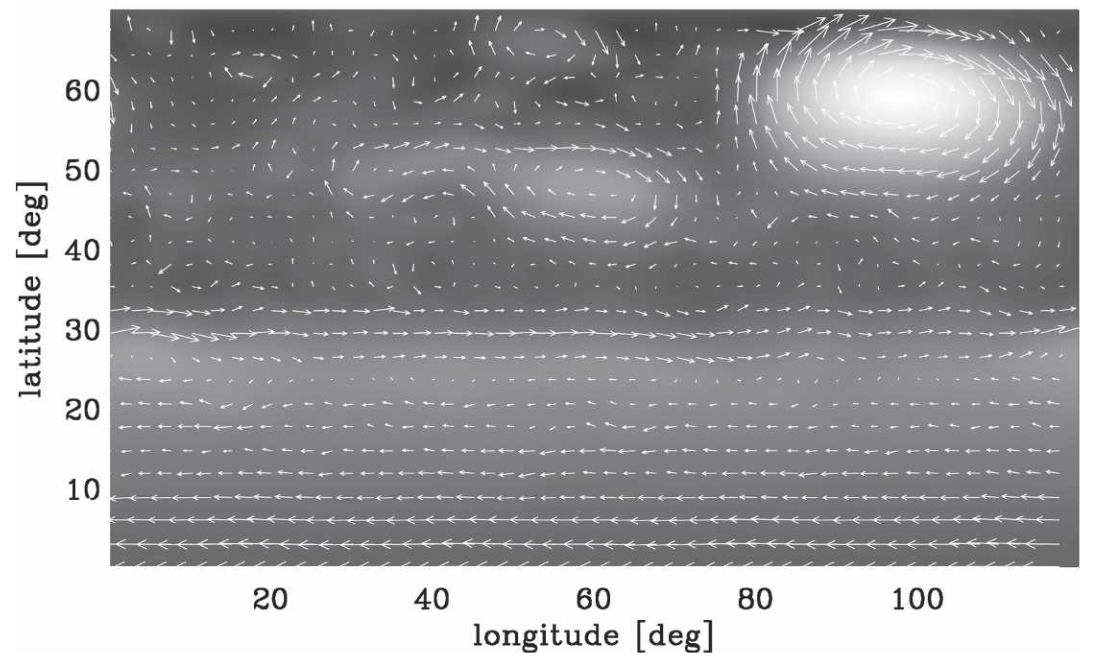
\includegraphics[clip,width=10cm]{./fig/intro/fig3.png}
    \caption{
      \footnotesize{\cite{Showman2007}のジオポテンシャルと
速度ベクトルの計算結果(4190地球日,中緯度の変形半径 : $L_d \sim 1200$ km).
      }
    }
    \label{fig3}
  \end{center}
\end{figure}
%
\subsection{Brueshaber et al. (2019)}
\label{sec:intro22}
\cite{Brueshaber2019}は\cite{Showman2007}の雷雲を
想定した強制浅水実験を極域(等緯度線で$\sim 60^\circ$ より高緯度)で計算し,
極渦とそのレジームに注目した.
その結果,図\ref{fig4}に示すようにBurger 数 : $Bu = (L_d/a)^2$ と呼ばれる無次元量の値によって,
極渦のレジームが変化することがわかった.
\begin{figure}[ht]
  \begin{center}
    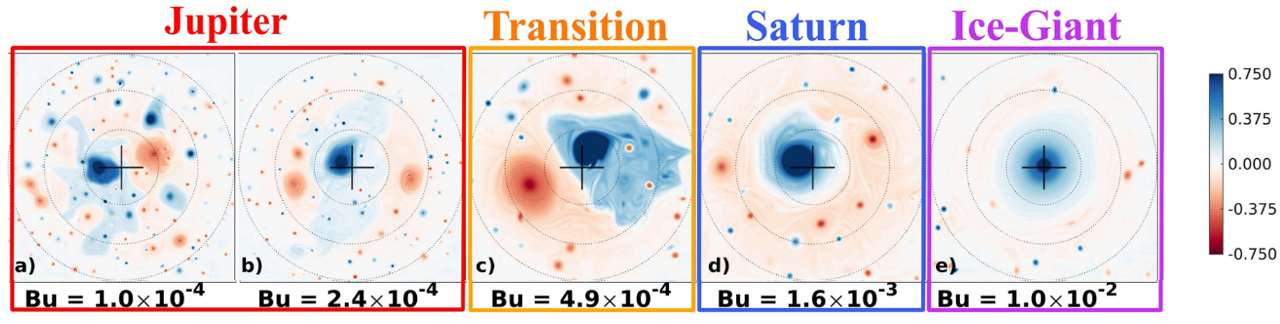
\includegraphics[clip,width=13cm]{./fig/intro/fig4.png}
    \caption{
      \footnotesize{\cite{Brueshaber2019}
      }
    }
    \label{fig4}
  \end{center}
\end{figure}


\section{研究目的}
\label{sec:intro3}


\setcounter{table}{0}
\setcounter{figure}{0}

\chapter{モデルと手法}
\section{支配方程式系}
\label{sec:model1}
本研究では球面上の1.5層浅水方程式系を用いる.
これは\cite{Showman2007}で用いられたモデルと同じである.
このモデルにおいて上層と下層はそれぞれの層で密度一定であり,
上層は活動的な層,下層は無限に深く静止したそうであると仮定する.
上層に対する運動量方程式と質量保存の式は
%
\begin{align}
& \DD{\Dvect{u}}{t}+ g' \Dgrad h + f \Dvect{k} \times \Dvect{u} = -\Dvect{D}_{\Dvect{u}},  \label{eq:eq1} \\
& \DP{g'h}{t} + \Ddiv (g'h\Dvect{u}) = \Sigma S_{storm} + S_{rad} - D_h. \label{eq:eq2} 
\end{align}
%
ここで,$D$は数値粘性項,$h$は上層の厚さ,$g'$は低減重力加速度, $S_{storm}$は雷雲を模した質量強制項,$S_{rad}$ は
放射緩和項である.
%\footnote{連続の式はBrueshaber et al. (2019) の記載が誤植と考え,Showman (2007) の記載を用いる.}
それぞれの強制項は
\begin{align}
&S_{storm} = s \cdot \exp \left [- \frac{R^2}{R_{storm}^2} - \frac{(t-t_0)}{\tau_{storm}^2} \right ], \label{eq:eq3}\\
&S_{rad}  = - \frac{\langle g'h \rangle - g'h_{eq}}{\tau_{mass}} - \frac{g'h - \langle g'h \rangle}{\tau_{APE}} \label{eq:eq4}
\end{align}
である.
%
%ここで,$s$は質量強制の最大値で$\pm 5.0, \pm 2.5, \pm 1.0$ の3つの値を用いる.
%またその正負の割合を$\alpha$とする.つまり$\alpha=1.0$ のとき,
%どのストームの$s$も正(高気圧性のストームが発生する).
%$R$は雷雲の中心位置からの距離,$R_{storm}$は雷雲の半径,
%$t$は雷雲が発生してからの時間,$t_0$は雷雲がピークを迎える時間,
%$\tau_{storm}$はストームの特徴的な時間スケール,
%$\langle \rangle$ はその瞬間の水平平均,
%$h_{eq}$は平衡状態での厚さ,
%$\tau_{mass}$はエネルギーに影響を与えず,$\langle h \rangle $を$h_{eq}$に向かって平衡化するときの時間スケール,
%$\tau_{APE}$は質量に影響を与えず,$h$を$\langle h \rangle$に向かって平衡化するときの時間スケールである.
%\cite{Brueshaber2019} ではこれらの強制項に加え,加えた質量強制を層から差し引く
%質量調整項を加えていたが,ここでは加えない.


\section{実験手法・実験設定}
\label{sec:model2}

\clearpage
\setcounter{table}{0}
\setcounter{figure}{0}

\chapter{実験結果}
\chapter{考察}
\chapter{結論}
sss


%\chapter*{付録}
\markright{付録 A}
\addcontentsline{toc}{chapter}{付録 A}
sss


%\chapter*{謝辞}
\markright{謝辞}
\addcontentsline{toc}{chapter}{謝辞}


\markright{参考文献}
\addcontentsline{toc}{chapter}{参考文献}
\bibliographystyle{abbrvnat}
\nocite{*}
\bibliography{./reference/reference}

\end{document}
